\documentclass[10pt,a4paper]{article}
\usepackage[latin1]{inputenc}
\usepackage[spanish]{babel}
\usepackage[toc, page, header]{appendix}
\renewcommand{\appendixtocname}{Apendices}
\renewcommand{\appendixpagename}{Apendices}
\usepackage{amsmath}
\usepackage{amsfonts}
\usepackage{amssymb}
\usepackage{graphicx}
\usepackage{url}
\author{Santiago Videla}
\title{Especificaci\'on de Requerimientos de Software}
\pagestyle{headings}
\begin{document}
\maketitle
\pagebreak
\tableofcontents
\pagebreak

\section{Introducci\'on}
  \subsection{Prop\'osito}
  \paragraph{}
  El prop\'osito de este documento es la especificaci\'on de requerimientos de software en el marco de la tesis de grado de la carrera Lic. en Cs. de la Computaci\'on de la FaMAF - UNC, \textbf{``Dise\~no de vacunas atenuadas con menor probabilidad de sufrir reversi\'on a la virulencia''}. Los requerimientos del software son provistos por integrantes de FuDePAN en su car\'acter de autores intelectuales de la soluci\'on que se pretende implementar y colaboradores de dicha tesis.

  \paragraph{}
  A continuaci\'on se enumeran las personas involucradas en el desarrollo de la tesis y que por lo tanto, representan la principal audiencia del presente documento.
  \begin{itemize}
  \item Dra. Laura Alonso Alemany: Directora de tesis, FaMAF
  \item Daniel Guston: Colaborador de tesis, FuDePAN
  \item Santiago Videla: Tesista, FaMAF
  \end{itemize}  
 
  \subsection{Alcance}
  El producto que se especifica en este documento se denomina \textbf{``vac-o''} y su principal objetivo es encontrar secuencias gen\'omicas de pat\'ogenos que mantengan funcionalidad como vacunas con una probabilidad m\'inima de sufrir reversi\'on a la virulencia. El producto final debe proveer al usuario, la capacidad de hacer uso del software mediante extensiones o \textit{plugins} que implementen las caracter\'isticas particulares para cada pat\'ogeno. 
  
  La principal responsabilidad de vac-o es la de proveer a las extensiones, un motor combinatorio de secuencias gen\'omicas utilizando diferentes estrategias computacionales que conduzcan a la optimizaci\'on de los c\'alculos. Por otro lado, las extensiones son responsables de evaluar las secuencias generadas asignando un puntaje a cada una con el fin de que vac-o genere el listado de secuencias resultante.

  En su versi\'on inicial, vac-o incluye una extensi\'on para la vacuna Sabin contra la poliomielitis que tambi\'en se especifica en este documento y podr\'ia ser tomada como gu\'ia para futuras extensiones.

  \subsection{Descripci\'on general del documento}
  La estructura de este documento sigue las recomendaciones de la ``Gu\'ia para la especifiaci\'on de requerimientos de la IEEE'' (IEEE Std 830-1998).

  En la secci\'on \ref{section-desc-gral} se presenta una descripci\'on general de vac-o, sus principales funcionalidades, interfaces y perfiles de usuarios.
  
  En la secci\'on \ref{section-req} se detallan los requerimientos funcionales espec\'ificos de vac-o y los principales atributos que debe cumplir el software. Adem\'as se incluye la especificaci\'on de una extensi\'on para la vacuna Sabin contra la poliomielitis.

\section{Descripci\'on General}
  \label{section-desc-gral}
  \subsection{Perspectiva del Producto}   
    Al momento de la confecci\'on de este documento, no existen productos de software que brinden las funcionalidades que se pretenden implementar. En este sentido, vac-o representa una innovaci\'on en el \'area de las bioinformaticas, cuyo principal objetivo es la optimizaci\'on de vacunas basadas en virus atenuados.
    
    Uno de los problemas de estas vacunas es su potencialidad de revertir a la virulencia. En sucesivas replicaciones, los virus atenuados pueden acumular mutaciones que les devuelvan el car\'acter patog\'enico y de esa manera podr\'ian producir enfermedad en el vacunado o sus contactos.
    
    Para lograr su objetivo, vac-o debe ser capaz de encontrar las variantes del virus con menor probabilidad de revertir a la patogenia. Partiendo de la secuencia gen\'omica que se encuentra en la cepa vacunal, se deben buscar las modificaciones de esta secuencia que cumplan las siguientes propiedades:
    \begin{itemize}
      \item Que originen una respuesta inmune protectora contra el virus salvaje.
      \item Que tengan muy baja probabilidad de mutar hasta convertirse en un virus pat\'ogeno.
    \end{itemize}
    
    Entre todas las secuencias encontradas, vac-o debe construir una lista o \textit{ranking} de secuencias con sus respectivos puntajes. Para lograr esto, se deber\'a implementar un \textit{plugin} que brinde la informaci\'on y las caracter\'isticas propias del virus. En particular, cada \textit{plugin} debe especificar las regiones combinatorias de inter\'es y ser capaz de asignar un puntaje a cada secuencia compar\'andola con la secuencia original. 

    En la figura~\ref{fig:1} se presenta el flujo de trabajo y funcionamiento general de vac-o. Notar que este esquema es puramente conceptual y no hace ninguna referencia a los detalles de implementaci\'on. La intenci\'on es clarificar al lector los diferentes ``actores'' y sus responsabilidades.
    \begin{figure}
	    \centering
	    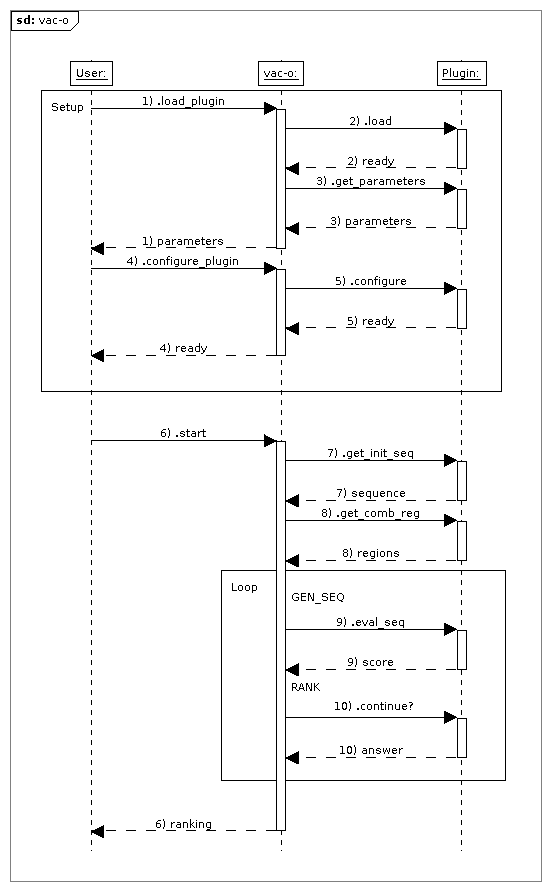
\includegraphics[scale=0.65]{seq-diagram.png}
	    \caption{Flujo de trabajo de vac-o}
	    \label{fig:1}
    \end{figure}

    \subsubsection{Interfaces del Sistema}
    No se registran requerimientos.

    \subsubsection{Interfaces de Usuario}
    La interfaz con el usuario final consiste de dos formularios y un listado con las secuencias resultantes. Inicialmente, el usuario de vac-o deber\'a indicar la ubicaci\'on o \textit{path} de la extensi\'on que desea usar. El siguiente paso, sera completar un formulario con los datos requeridos por la extensi\'on elegida. Finalmente, se da comienzo a la ejecuci\'on y se recibe como resultado, la lista de secuencias con sus respectivos puntajes.

    \subsubsection{Interfaces de Hardware}
    No se registran requerimientos.

    \subsubsection{Interfaces de Software}
    \begin{itemize}
      \item BioPP: Se debe utilizar la librer\'ia BioPP para realizar el \textit{folding} de secuencias gen\'omicas, predicci\'on de la estructura secundaria y c\'alculo de distancias.
      \item Boost.Python: Se debe utilizar Boost.Python para brindar a los desarrolladores de extensiones, la posibilidad de hacerlo utilizando el lenguaje de programaci\'on Python.
      \item QT: Se debe utilizar QT para el desarrollo de la interfaz de usuario.
    \end{itemize}

    \subsubsection{Interfaces de Comunicaciones}
    No se registran requerimientos.

    \subsubsection{Restricciones de Memoria}
    No se registran restricciones de memoria para la ejecuci\'on del software. No obstante, se debe tener en cuenta que dada la naturaleza y la complejidad del problema, el tiempo de calculo estar\'a directamente relacionado con la memoria disponible.

    \subsubsection{Operaciones}
    No se registran requerimientos.

    \subsubsection{Requerimientos de Instalaci\'on}
    No se registran requerimientos.

  \subsection{Funciones del Producto}
  
  \subsubsection{Configuraci\'on inicial}
  Inicialmente, vac-o presenta al usuario final una pantalla con un formulario donde el usuario debe indicar la ubicaci\'on de la extensi\'on que desea usar. A continuaci\'on, vac-o carga la extensi\'on en memoria y presenta al usuario otro formulario con los campos requeridos por la extensi\'on cargada.
  Una vez que los datos son validados, vac-o configura la extensi\'on con los valores enviados por el usuario y queda listo para comenzar la ejecuci\'on cuando el usuario lo indique.

  \subsubsection{Configuraci\'on de vac-o}
  Antes de dar comienzo a la generaci\'on de secuencias gen\'omicas, vac-o debe solicitar a la extensi\'on cargada los siguientes valores:
  \begin{itemize}
    \item Secuencia inicial: La secuencia gen\'omica que se encuentra en la cepa vacunal y se desea mejorar.
    \item Regiones combinatorias: Las regiones de la secuencia inicial que resultan de interes, indicando sus posiciones de inicio y fin, y que tipo de regiones son cada una (restricciones en base a c\'odigo gen\'etico, o en base a estructura secundaria).
    \item Estrategias de busqueda: La estrategia que se debe utilizar para la generaci\'on o busqueda de nuevas secuencias.
  \end{itemize}
  
  \subsubsection{Generaci\'on de secuencias}
  Luego de las configuraciones basicas, vac-o esta en condiciones de generar nuevas secuencias gen\'omicas que cumplan las restricciones que hallan sido impuestas. Para esto, se deben calcular las posibles ``mutaciones'' de cada region combinatoria (teniendo en cuenta el tipo de regi\'on y sus posibles intersecciones) y de acuerdo a la estrategia de busqueda, construir nuevas secuencias que seran evaluadas posteriormente por la extensi\'on. Dado que el espacio de busqueda podr\'ia ser eventualmente muy grande, el criterio de parada para la generaci\'on de secuencias tambi\'en debe ser provisto por la extensi\'on.

  Notar que esta funcionalidad es el ``corazon'' de vac-o y es donde se encuentra la mayor complejidad del problema a resolver. 

  Supongamos $N \geqslant 1$ y $R_{1}, \cdots, R_{N}$ regiones combinatorias. Luego, tendremos: \\
  \begin{center}    
    $M_{1\cdot1},..., M_{1\cdot j_{1}}$ mutaciones de $R_{1}$\\ 
    $M_{2\cdot1},..., M_{2\cdot j_{2}}$ mutaciones de $R_{2}$\\
    $\cdots$ \\
    $M_{N\cdot1},..., M_{N\cdot j_{N}}$ mutaciones de $R_{N}$   
  \end{center}
  con $j_{1}, \cdots, j_{N} \geqslant 1$. Es decir, que el n\'umero de posibles secuencias que vac-o ``deberia'' evaluar sera igual al producto $j_{1} \times j_{2} \times \cdots \times j_{N}$. 

  Haciendo uso de diferentes estrategias de busqueda, combinadas con las funciones de evaluaci\'on provistas por la extensi\'on, vac-o intentara optimizar esta generaci\'on de secuencias.

  \subsubsection{Evaluaci\'on de secuencias}
  De acuerdo a los puntajes asignados por la extensi\'on a cada una de las secuencias generadas, vac-o debe construir un listado o \textit{ranking} de secuencias que sera dado al usuario como resultado final de la ejecuci\'on.

  \subsection{Caracter\'isticas de Usuarios}
  Se identifican 3 tipos de usuarios de vac-o:
  \begin{itemize}
    \item Final: que solo interact\'ua a trav\'es de la interfaz gr\'afica.
    \item Extensionista: que posee los conocimientos de programaci\'on suficientes como para implementar extensiones de vac-o. A los fines de ampliar los potenciales usuarios dentro de esta categor\'ia, es que se ofrece la posibilidad de desarrollar extensiones usando el lenguaje Python.
    \item Contribuidor: que contribuye al c\'odigo fuente de vac-o realizando mejoras o desarrollando nuevas funcionalidades.
  \end{itemize}

  \subsection{Restricciones}
  El producto debe ser desarrollado utilizando el lenguaje de programaci\'on C++ y bajo la licencia de software GPLv3.
  
  \subsection{Suposiciones y Dependencias}
    \begin{itemize}
      \item Sistema operativo: GNU/Linux
    \end{itemize}
  
  \subsection{Trabajo Futuro}
  Probablemente una de las principales mejoras a la primer versi\'on de vac-o, sera realizar las modificaciones necesarias para permitir la ejecuci\'on del software en paralelo y de esta manera reducir los tiempos de c\'alculo. 
  Por otro lado, se debera profundizar en el desarrollo de extensiones para diferentes tipos de vacunas y virus.
  

\section{Requerimientos}
  \label{section-req}  
  \subsection{Funciones del Sistema}

  \subsubsection{Configuraci\'on inicial}
  El objetivo de esta funci\'on es la carga en memoria de la extensi\'on que se desea utilizar para ejecutar vac-o.
  \begin{enumerate}
    \item \textbf{Carga de la extensi\'on:}
    El sistema recibe la ubicaci\'on del archivo \textit{.so} y lo carga en memoria. Si la carga es exitosa, se devuelven los parametros requeridos por la extensi\'on (\textit{[(nombre, tipo, validaciones, defecto)]}) para su posterior configuraci\'on. En caso de que la carga de la extensi\'on fracase, se devuelve un mensaje de error.
    
    \item \textbf{Validaci\'on de valores:}
    La interfaz de usuario (QT) es responsable de la validaci\'on de los datos ingresados por el usuario para la configuraci\'on de la extensi\'on. Para esto, se deberan usar los diferentes \textit{criterios de validaci\'on} para cada parametro y solo cuando la validaci\'on sea exitosa, los valores son enviados al sistema. Caso contrario, se debe presentar un mensaje de error al usuario.
    
    \item \textbf{Configuraci\'on de la extensi\'on:}
    El sistema recibe la lista de parametros requeridos por la extensi\'on (\textit{[(nombre, valor)]}) y se asignan los valores en la extensi\'on. Finalmente, se devuelve un mensaje de exito indicando que vac-o esta listo para comenzar la ejecuci\'on.
  \end{enumerate}

  \subsubsection{Configuraci\'on de vac-o}
  El objetivo de esta funci\'on es solicitar a la extensi\'on cargada en memoria, la informaci\'on necesaria para comenzar la ejecuci\'on del motor combinatorio.
  \begin{enumerate}
    \item \textbf{Secuencia inicial:}
    El sistema solicita a la extensi\'on cargada en memoria, la secuencia de ARN que se desea optimizar. La extensi\'on debe devolver la secuencia en formato FASTA y el sistema la almacena en memoria.
    
    \item \textbf{Regiones combinatorias:}
    El sistema solicita a la extensi\'on cargada en memoria, las regiones combinatorias de interes para la optimizaci\'on. La extensi\'on debe devolver las regiones (\textit{[(inicio, fin, tipo, evaluador)]}) y el sistema inicializa cada region en memoria. Para cada region, el parametro \textit{tipo} debe ser uno de los siguientes:
    \begin{itemize}
      \item Estructura secundaria (SS): Las posibles mutaciones de la region deben conservar la estructura secundaria.
      \item Codigo genetico (GC): Las posibles mutaciones de la region deben resultar silentes en t\'erminos de expresi\'on aminoc\'idica.
      \item Personalizada (CU): La extensi\'on debe proporcionar la implementaci\'on de la region combinatoria.
    \end{itemize}

    El parametro \textit{evaluador} debe ser una funci\'on $f: Secuencia \rightarrow (0,1)$ que sera utilizada por el sistema para determinar la ``bondad'' de las diferentes mutaciones de cada region.

    \item \textbf{Estrategia de busqueda:}
    El sistema solicita a la extensi\'on un \textit{umbral} de ``bondad'' y debe implementar diferentes estrategias de optimizaci\'on, asegurando que se cumpla lo siguiente:

    Sea $n$ el numero de regiones combinatorias, $s_{i}$ la secuencia seleccionada de la region $i$ y $f_{i}: Secuencia \rightarrow (0,1)$ la funci\'on de evaluaci\'on de la region $i$, con $i=1, ..., n$.
    \begin{center}
    $\prod_{i=1}^{n} f_{i}(s_{i}) \ge umbral$
    \end{center}
    \item \textbf{Librerias externas:}
    El sistema solicita a la extensi\'on, la libreria con la que se deben generar las mutaciones de cada region combinatoria.
  \end{enumerate}

  \subsubsection{Generaci\'on de secuencias}
  El objetivo de esta funci\'on es la construcci\'on de nuevas secuencias gen\'omicas que cumplan con las restricciones impuestas.
  \begin{enumerate}
    \item \textbf{Generar mutaciones de region combinatoria:}
    Para cada region combinatoria, el sistema debe ser capaz de generar todas las posibles mutaciones que cumplan con las restricciones impuestas por el tipo de region y considerando las posibles intersecciones con las demas regiones.
    
    \item \textbf{Generar secuencias:}
    A partir de las mutaciones de cada region combinatoria, se deben construir nuevas secuencia gen\'omicas, reemplazando cada region por su mutaci\'on en la secuencia inicial y asegurar que la secuencia resultante consereve la estructura secundaria de la secuencia inicial. El criterio de terminaci\'on en la generaci\'on de secuencias debe ser provisto por la extensi\'on.

    \item \textbf{Validaci\'on de secuencias:}
    Para cada secuencia generada por el sistema, se deben aplicar pruebas de ``calidad''. El sistema solicita a la extensi\'on el tipo de prueba, que sera uno de los siguientes:
      \begin{itemize}
        \item Mutaciones sistem\'aticas.
	\item Mutaciones al azar.
      \end{itemize}
    y el tipo de criterio, que sera uno de los siguientes:
      \begin{itemize}
        \item Comparaci\'on estructural por regiones.
	\item Conteo y comparaci\'on de nucle\'otidos apareados/desapareados.
      \end{itemize}
    Luego, la validaci\'on consiste en aplicar el criterio de calidad a las $N$ mutaciones obtenidas. Las secuencias que no pasen las pruebas de calidad seran descartadas.
  \end{enumerate}

  \subsubsection{Evaluaci\'on de secuencias}
  El objetivo de esta funci\'on es la evaluaci\'on y posterior construcci\'on de un \textit{ranking} de secuencias gen\'omicas.
  \begin{enumerate}    
    \item \textbf{Asignar puntaje a una secuencia:}
    El sistema solicita a la extensi\'on cargada en memoria, un puntaje para una secuencia dada. La extensi\'on debe evaluar la secuencia recibida comparandola con la secuencia inicial y devolver un puntaje.
    
    \item \textbf{Construir \textit{ranking} de secuencias:}
    El sistema debe construir un \textit{ranking} de secuencias basandose en los puntajes asignados por la extensi\'on. Este listado de secuencias es adem\'as, la salida final de la ejecuci\'on.
  \end{enumerate}

  \subsection{Restricciones de Rendimiento}
  No se registran requerimientos.

  \subsection{Base de Datos}
  No se registran requerimientos.

  \subsection{Restricciones de Dise\~no}
    \subsubsection{Cumplimiento de Est\'andares}
    El producto debe cumplir con los siguientes principios y patrones de dise\~no de la programaci\'on orientada a objetos. Los primeros 5, son tambi\'en conocidos por el acr\'onimo ``\textbf{SOLID}''.
    \begin{itemize}
      \item \textbf{S}ingle responsibility principle (SRP)
      \item \textbf{O}pen/closed principle (OCP)
      \item \textbf{L}iskov substitution principle (LSP)
      \item \textbf{I}nterface segregation principle (ISP)
      \item \textbf{D}ependency inversion principle (DIP)   
      \item Law of Demeter (LoD)
    \end{itemize}

    Adem\'as el producto debe cumplir con el estandar ANSI C++ y el ``coding style'' provisto por FuDePAN.

  \subsection{Atributos del Software}
    Se requiere que el c\'odigo del producto tenga un 80\% de covertura con pruebas automatizadas.

\pagebreak

\begin{appendices} 
  \section{Definiciones, Acr\'onimos y Abreviaturas}
  \label{appendix-def}
  \begin{itemize}
    \item \textbf{vac-o}: Combinatory Vaccine Optimizer.
    \item \textbf{FaMAF}: Facultad de Matem\'atica, Astronom\'ia y F\'isica.
    \item \textbf{UNC}: Universidad Nacional de C\'ordoba.
    \item \textbf{FuDePAN}: Fundaci\'on para el Desarrollo de la Programaci\'on en \'Acidos Nucleicos.
    \item \textbf{API}: Application Programming Interface.
    \item \textbf{GPL}: General Public License.
    \item \textbf{IEEE}: Institute of Electrical and Electronics Engineers
    \item \textbf{SOLID}: acr\'onimo nemot\'ecnico introducido por Robert C. Martin en la d\'ecada de 2000, que representa cinco principios b\'asicos de programaci\'on y dise\~no orientado a objetos.
    \item \textbf{LoD}: Law of Demeter, principio de dise\~no orientado a objetos para lograr ``bajo acoplamiento''.    
    \end{itemize}
  \section{Referencias}
  \label{appendix-ref}
  \begin{itemize}
    \item C++: Lenguaje de programaci\'on. \\
    \url{http://www.cplusplus.com}
    \item Python: Lenguaje de programaci\'on interpretado.\\ 
    \url{http://www.python.org}
    \item BioPP: Librer\'ia C++ para biolog\'ia molecular\\
    \url{http://code.google.com/p/biopp}
    \item Boost.Python: Librer\'ia C++ para la interacci\'on con Python.\\
    \url{http://www.boost.org/doc/libs/1_42_0/libs/python/doc/index.html}
    \item QT: Librer\'ia C++ para el desarrollo de interfaces gr\'aficas.\\
    \url{http://qt.nokia.com/products}
    \item GPL: General Public License. \\
    \url{http://www.gnu.org/licenses/gpl.html}
    \item IEEE STD 830-1998: Gu\'ia para la especifiaci\'on de requerimientos. \\
    \url{http://standards.ieee.org/reading/ieee/std_public/description/se/830-1998_desc.html}
    \item SOLID: ``Design Principles and Design Patterns'', Robert C. Martin. \\
    \url{http://www.objectmentor.com/resources/articles/Principles_and_Patterns.pdf}    
    \item FASTA: Formato basado en texto, utilizado para representar secuencias gen\'omicas.\\
    \url{http://es.wikipedia.org/wiki/Formato_FASTA}
  \end{itemize}
     
\end{appendices}

\end{document}
